\documentclass[11pt,a4paper,final]{article} %draft

\usepackage[T1,T2A]{fontenc}
\usepackage[utf8]{inputenc}
\usepackage[english, russian]{babel}

\usepackage[final]{pdfpages}

\usepackage{textcomp,enumitem}

\usepackage{amsmath,amsthm,amssymb}

\usepackage{fancyhdr} % для настройки страницы и колонтитулов

\usepackage{graphicx}

\usepackage{indentfirst} % автоматический отступ в начале каждого раздела

\usepackage[unicode, pdftex, colorlinks, urlcolor=blue]{hyperref}

\usepackage[left=2cm,right=2cm,top=2cm,bottom=2cm,bindingo ffset=0cm]{geometry}

\linespread{1.3} % устанавливает междустрочный интервал

\pagestyle{plain} % для отображения номеров внизу 

\usepackage{float}

\usepackage{listings} 

\usepackage{pdflscape}
\usepackage{listings} 
\definecolor{darkgreen}{rgb}{0,0.5,0}

\lstset{
backgroundcolor=\color{white},  % Устанавливаем белый фон для блока кода
basicstyle=\ttfamily\small\fontfamily{inconsolata}\selectfont,  % Основной стиль текста: моноширинный шрифт Inconsolata с небольшим размером
commentstyle=\color{darkgreen}\slshape,  % Комментарии будут зелеными и курсивными
keywordstyle=\color{blue}\bfseries,  % Ключевые слова выделяются синим цветом и полужирным шрифтом
numberstyle=\scriptsize\color{gray},  % Стиль нумерации строк: маленький размер шрифта и серый цвет
stringstyle=\color{orange},  % Строки (текст в кавычках) отображаются оранжевым цветом
breakatwhitespace=false,  % Не прерывать строки только по пробелам
breaklines=true,  % Автоматический перенос длинных строк
postbreak=\mbox{\textcolor{gray}{$\hookrightarrow$}}, % Символ переноса строки
captionpos=b,  % Позиция заголовка/описания для блока кода — внизу (b — bottom)
keepspaces=true,  % Сохранить пробелы, как они есть, в исходном коде
numbers=left,  % Нумерация строк будет отображаться слева
numbersep=5pt,  % Отступ между строками кода и номерами строк (4pt)
showspaces=false,  % Не показывать пробелы
showstringspaces=false,  % Не показывать пробелы внутри строк
showtabs=false,  % Не показывать символы табуляции
tabsize=4,  % Размер табуляции — 4 пробела
language=sql,  % Указываем язык программирования для синтаксического подсветки
captionpos=t,  % Заголовок кода будет размещен вверху (t — top)
xleftmargin=0mm,  % Убираем отступ слева
frame=single,  % Однотонная рамка вокруг блока кода
framerule=0.25mm,  % Толщина рамки — 0.25 мм
literate=
{а}{{\selectfont\char224}}1
{б}{{\selectfont\char225}}1
{в}{{\selectfont\char226}}1
{г}{{\selectfont\char227}}1
{д}{{\selectfont\char228}}1
{е}{{\selectfont\char229}}1
{ж}{{\selectfont\char230}}1
{з}{{\selectfont\char231}}1
{и}{{\selectfont\char232}}1
{й}{{\selectfont\char233}}1
{к}{{\selectfont\char234}}1
{л}{{\selectfont\char235}}1
{м}{{\selectfont\char236}}1
{н}{{\selectfont\char237}}1
{о}{{\selectfont\char238}}1
{п}{{\selectfont\char239}}1
{р}{{\selectfont\char240}}1
{с}{{\selectfont\char241}}1
{т}{{\selectfont\char242}}1
{у}{{\selectfont\char243}}1
{ф}{{\selectfont\char244}}1
{х}{{\selectfont\char245}}1
{ц}{{\selectfont\char246}}1
{ч}{{\selectfont\char247}}1
{ш}{{\selectfont\char248}}1
{щ}{{\selectfont\char249}}1
{ъ}{{\selectfont\char250}}1
{ы}{{\selectfont\char251}}1
{ь}{{\selectfont\char252}}1
{э}{{\selectfont\char253}}1
{ю}{{\selectfont\char254}}1
{я}{{\selectfont\char255}}1
{А}{{\selectfont\char192}}1
{Б}{{\selectfont\char193}}1
{В}{{\selectfont\char194}}1
{Г}{{\selectfont\char195}}1
{Д}{{\selectfont\char196}}1
{Е}{{\selectfont\char197}}1
{Ж}{{\selectfont\char198}}1
{З}{{\selectfont\char199}}1
{И}{{\selectfont\char200}}1
{Й}{{\selectfont\char201}}1
{К}{{\selectfont\char202}}1
{Л}{{\selectfont\char203}}1
{М}{{\selectfont\char204}}1
{Н}{{\selectfont\char205}}1
{О}{{\selectfont\char206}}1
{П}{{\selectfont\char207}}1
{Р}{{\selectfont\char208}}1
{С}{{\selectfont\char209}}1
{Т}{{\selectfont\char210}}1
{У}{{\selectfont\char211}}1
{Ф}{{\selectfont\char212}}1
{Х}{{\selectfont\char213}}1
{Ц}{{\selectfont\char214}}1
{Ч}{{\selectfont\char215}}1
{Ш}{{\selectfont\char216}}1
{Щ}{{\selectfont\char217}}1
{Ъ}{{\selectfont\char218}}1
{Ы}{{\selectfont\char219}}1
{Ь}{{\selectfont\char220}}1
{Э}{{\selectfont\char221}}1
{Ю}{{\selectfont\char222}}1
{Я}{{\selectfont\char223}}1,
numbers=left, % пронумеровать строки с левой стороны
breaklines=true % разрешает автоматический перенос строк
}

\hypersetup{
colorlinks=true, % делает ссылки цветными вместо рамки
linkcolor=blue, % цвет внутренних ссылок
urlcolor=blue, % цвет внешних ссылок
citecolor=blue % цвет ссылок на литературу в тексте
}
\textheight=24cm 
\textwidth=16cm
\oddsidemargin=0pt 
\topmargin=-1.5cm
\parindent=24pt 
\parskip=0pt 
\tolerance=2000 
\flushbottom 

%\usepackage[font=scriptsize]{caption}
\usepackage[labelsep=period]{caption}

\usepackage{amsmath}
\usepackage{multirow} 
\usepackage{tabularx}
\usepackage{titlesec}

% Настройка дополнительного уровня заголовков
\setcounter{secnumdepth}{4} % Увеличиваем глубину нумерации
\setcounter{tocdepth}{4}    % Увеличиваем глубину оглавления

% Настройка стиля для \subsubsubsection
\titleformat{\paragraph}[block] % "runin" делает заголовок частью текста
{\normalfont\normalsize\bfseries}{\theparagraph}{1em}{} 


\newcommand{\specialcell}[2][l]{\begin{tabular}[#1]{@{}l@{}}#2\end{tabular}}

\begin{document}

\thispagestyle{empty}

\begin{center}
	{\Large МИНОБРНАУКИ РОССИИ}\\
	~\\
	{\large ФЕДЕРАЛЬНОЕ ГОСУДАРСТВЕННОЕ БЮДЖЕТНОЕ ОБРАЗОВАТЕЛЬНОЕ УЧРЕЖДЕНИЕ ВЫСШЕГО ПРОФЕССИОНАЛЬНОГО ОБРАЗОВАНИЯ}\\
	~\\
	{\Large \bf <<САНКТ-ПЕТЕРБУРГСКИЙ ПОЛИТЕХНИЧЕСКИЙ УНИВЕРСИТЕТ ПЕТРА ВЕЛИКОГО>>}\\
	~\\
	{\large Институт компьютерных наук и кибербезопасности }\\
	{\large Высшая школа технологий искусственного интеллекта}\\
	{\large Направление 02.03.01 Математика и компьютерные науки}\\
	~\\
	~\\
	~\\
	~\\
	{\Large \bf  Отчет по лабораторным работам }\\
	\vspace{3mm}
	{\Large {по дисциплине <<Методы проектирования баз данных>>}}\\
	\vspace{3mm}
	~\\
	~\\
	~\\
	~\\
	~\\
	~\\
	{\large Обучающийся: \underline{\hspace{3.5cm}} \hspace{12mm} Шихалев А.О.}\\
	~\\
	{\large Руководитель: \underline{\hspace{3.5cm}} \hspace{12mm} Попов С.Г.}\\
	~\\
	~\\
	~\\
	~\\
	~\\
\end{center}
\begin{flushright}
	
	«\underline{\hspace{1cm}}»\underline{\hspace{3cm}}20\underline{\hspace{0.7cm}}г.
\end{flushright}
~\\
~\\
\begin{center}
	{\large Санкт-Петербург, 2024}
\end{center}

\newpage

\tableofcontents

\newpage
\section* {Введение}
\addcontentsline{toc}{section}{Введение}
В данном отчёте описан результат выполнения лабораторных работ, которые расширяют функциональные возможности базы данных <<Процесс прохождения кастинга претендентом на роль в фильме>>, которая была разработана в течение предыдущего семестрового курса <<Теоретические основы баз данных>>. 

\newpage
\section{Постановка задачи}
Необходимо выполнить 5 лабораторных работ:
\begin{enumerate}
	\item Создать представление, инкапсулирующее запрос. Продемонстрировать невозможность модификации представления, написать запрос, использующий в себе это представление.
	\item Создать таблицу подсчета количества заявок каждого актера. Написать триггеры, автоматизирующие сбор статистики в таблице.
	\item Создать двух пользователей: первый имеет доступ только на просмотр представления из первого задания, второй также может редактировать таблицы, участвующие в запросе представления.
	\item Процедуры и функции.
	\item Управление транзакциями.
\end{enumerate}

\newpage
\section{Лабораторные работы}
\subsection{Создание представления}

\textbf{Задача:} Разработать представление для хранения запроса внутри СУБД.

\textbf{Формулировка запроса:} Для каждого режиссера подсчитать общее количество фильмов, которые он срежиссировал, а также количество актеров, которые снимались в этих фильмах.

В результате реализации задачи было создано представление, хранящее в себе запрос, подсчитывающий для каждого режиссера общее количество снятых им фильмов и число актеров, которые снимались в этих фильмах. Код создания представления представлен в \hyperref[lst:l1]{листинге 1}.

\begin{lstlisting}[caption={Создание представления}, label=lst:l1]
CREATE VIEW director_view AS
	SELECT d.id_director, d.name, d.surname, 
	COUNT(DISTINCT f.id_film) AS film_count, 
	COUNT(DISTINCT act.id_actor) AS actor_count
	FROM director AS d
	JOIN film AS f ON d.id_director = f.id_director
	JOIN role AS r ON f.id_film = r.id_film
	JOIN application AS app ON r.id_role = app.id_role
	JOIN actor AS act ON app.id_actor = act.id_actor
	GROUP BY d.id_director, d.name, d.surname;
\end{lstlisting}

Получившееся представление (view) является виртуальной таблицей со следующими атрибутами:
\begin{itemize}
	\item id\_director - id режиссера;
	\item d.name - имя режиссера;
	\item d.surname - фамилия режиссера;
	\item film\_count - количество фильмов, снятых каждым режиссером;
	\item actor\_count - количество актеров, подавших заявки на роль в фильмах каждого режиссера.
\end{itemize}

Результат вывода представления представлен на \hyperref[fig:pic1]{рисунке 1.}

При попытке модификации таблицы выводятся ошибки, посколько представления не являются обновляемыми таблицами. 
Результат применения команд языка DML к созданному представлению представлен на \hyperref[fig:pic2]{рисунке 2.}

\newpage
\begin{figure}[H]
	\centering
	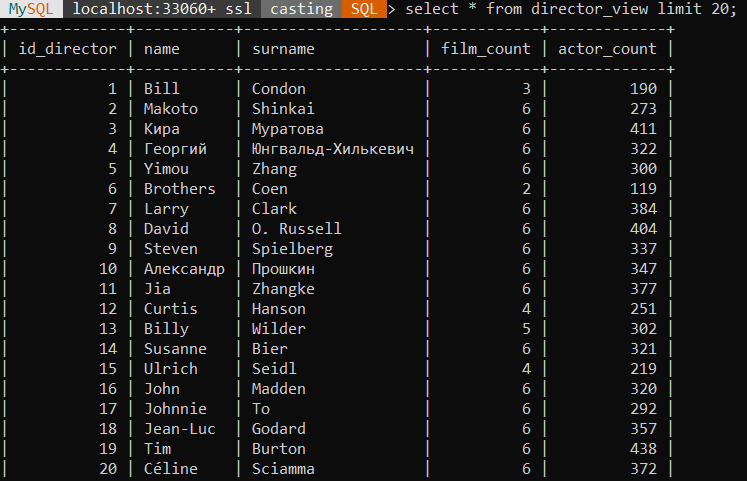
\includegraphics[width=0.8\linewidth]{pic1.png}
	\caption{Вывод представления}
	\label{fig:pic1}
\end{figure}

\begin{figure}[H]
	\centering
	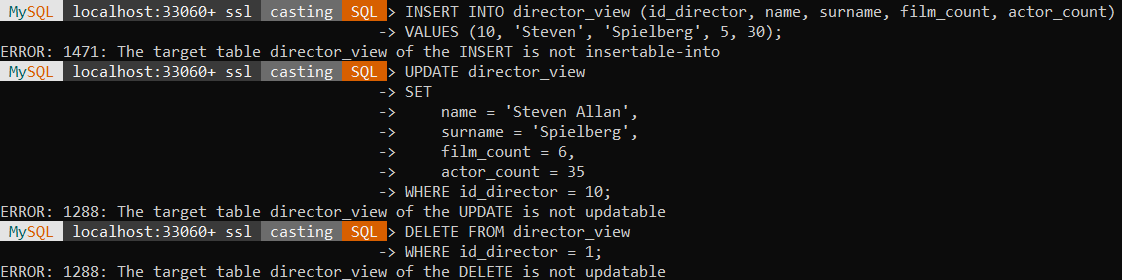
\includegraphics[width=0.9\linewidth]{pic2.png}
	\caption{Ошибки, возникающие при попытке модификации представления}
	\label{fig:pic2}
\end{figure}

\textbf{Задача:} Написать запрос, включающий в себя созданное представление.

\textbf{Формулировка запроса №1:} Получить общее количество жанров и ролей в фильмах каждого режиссера.

\par В результате реализации задачи был написан запрос, представленный в \hyperref[lst:l2]{листинге 2}.

\begin{lstlisting}[caption={Код запроса, использующего представление}, label=lst:l2]
SELECT dv.id_director, dv.name, dv.surname, dv.film_count, dv.actor_count, 
	COUNT(DISTINCT gnr.id_genres) AS count_genres,
	COUNT(DISTINCT role.id_role) AS count_role
FROM director_view as dv
JOIN film AS f ON dv.id_director = f.id_director
JOIN film_genres AS fg ON f.id_film = fg.id_film
JOIN genres AS gnr ON fg.id_genres = gnr.id_genres
JOIN role AS role ON f.id_film = role.id_film
GROUP BY dv.id_director, dv.name, dv.surname;
\end{lstlisting}

Результат выполнения запроса №1 представлен на \hyperref[fig:pic3]{рисунке 3.}

\begin{figure}[H]
	\centering
	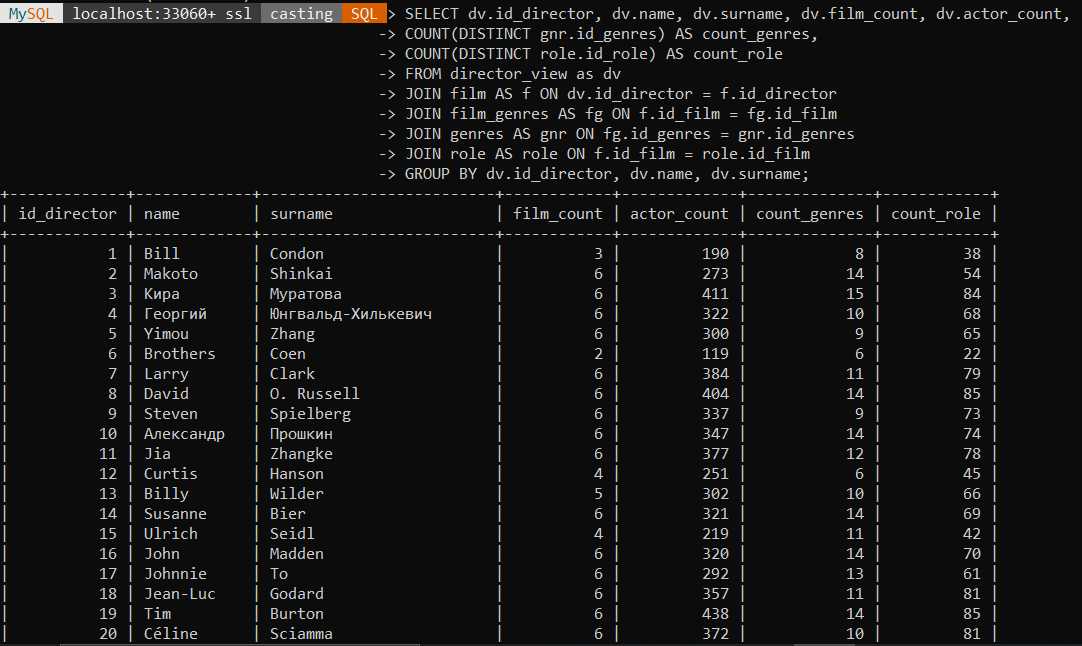
\includegraphics[width=0.9\linewidth]{pic3.png}
	\caption{Результат выполнения запроса №1}
	\label{fig:pic3}
\end{figure}


\textbf{Формулировка запроса №2:} Получить количество утвержденных заявок для фильмов каждого режиссера.

\par В результате реализации задачи был написан запрос, представленный в \hyperref[lst:l3]{листинге 3}.

\begin{lstlisting}[caption={Код запроса, использующего представление}, label=lst:l3]
SELECT dv.id_director, dv.name, dv.surname, dv.film_count, dv.actor_count, 
	COUNT(CASE WHEN du.getting_a_role = 'Роль получена' THEN 1 END) AS count_received_roles
FROM director_view as dv
JOIN film AS f ON dv.id_director = f.id_director
JOIN role AS role ON f.id_film = role.id_film
JOIN application AS app ON role.id_role = app.id_role
JOIN doubles_audition AS du ON app.id_application = du.id_application
GROUP BY dv.id_director, dv.name, dv.surname
ORDER BY dv.id_director ASC;
\end{lstlisting}

Результат выполнения запроса №2 представлен на \hyperref[fig:pic4]{рисунке 4.}

\newpage
\begin{figure}[H]
	\centering
	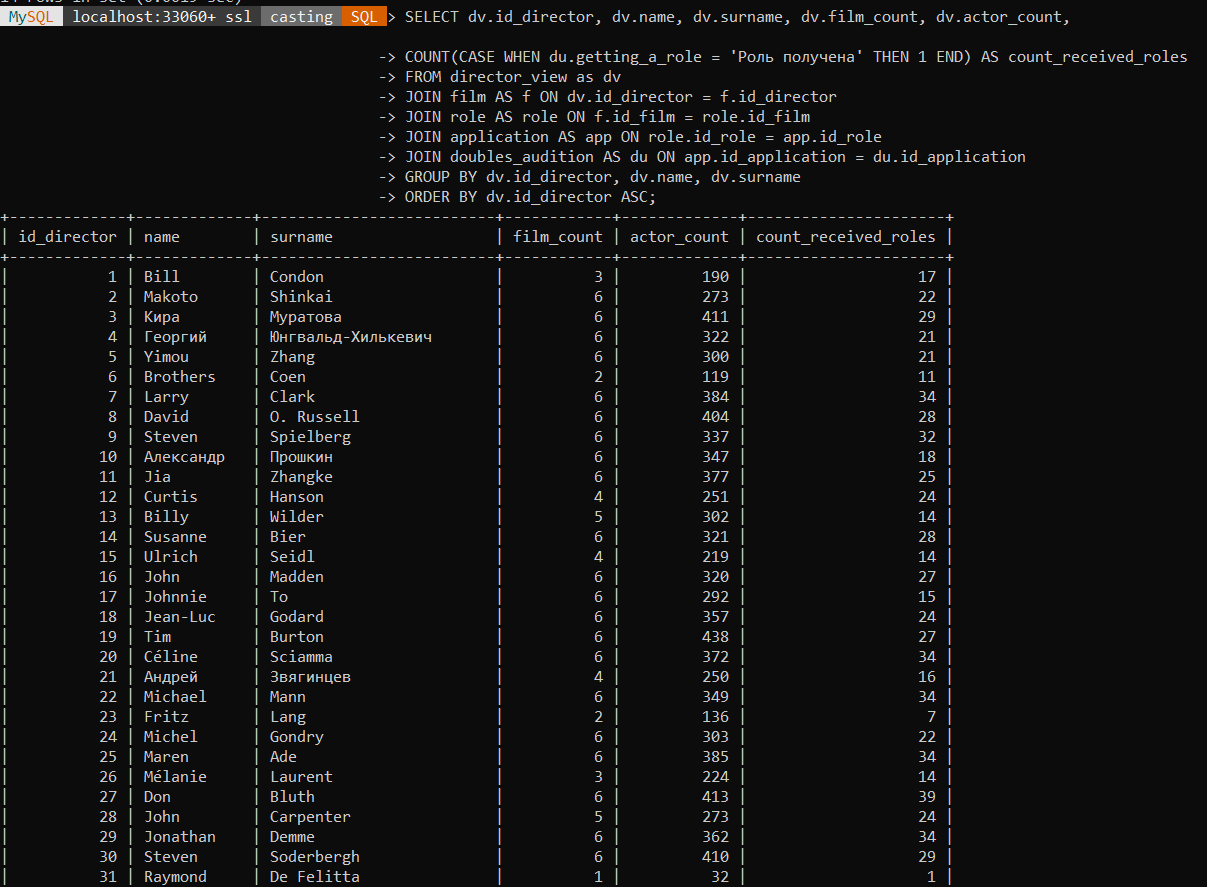
\includegraphics[width=0.9\linewidth]{pic4.png}
	\caption{Результат выполнения запроса №2}
	\label{fig:pic4}
\end{figure}


\subsection{Событийная модель, триггеры}
\textbf{Задача:} Создать таблицу подсчета количества заявок, поданных каждым актером. Для реализованной таблицы написать триггеры, автоматизирующие сбор статистики в таблице.

\par В результате реализации задачи была создана таблица \textbf{actor\_apps}. Код создания таблицы представлен в
\hyperref[lst:l4]{листинге 4}.

\begin{lstlisting}[caption={Код создания таблицы actor\_apps}, label=lst:l4]
CREATE TABLE IF NOT EXISTS actor_apps(
	id_actor int unsigned NOT NULL,
	surname varchar(30) COLLATE utf8mb4_unicode_ci DEFAULT NULL,
	name varchar(20) COLLATE utf8mb4_unicode_ci DEFAULT NULL,
	patronymic varchar(20) COLLATE utf8mb4_unicode_ci DEFAULT NULL,
	num_apps int unsigned NOT NULL, 
	PRIMARY KEY(id_actor)
)ENGINE=InnoDB DEFAULT CHARSET=utf8mb4 COLLATE=utf8mb4_unicode_ci;
\end{lstlisting} 

Полученная таблица была заполнена данными при помощи запроса, представленного в \hyperref[lst:l5]{листинге 5}.

\begin{lstlisting}[caption={Код заполнения таблицы actor\_apps}, label=lst:l5]
INSERT INTO actor_apps(id_actor, surname, name, patronymic, num_apps)
SELECT a.id_actor, a.surname, a.name, a.patronymic, 
	COUNT(DISTINCT app.id_application) AS num_apps
FROM actor AS a
JOIN application AS app ON a.id_actor = app.id_actor
GROUP BY a.id_actor; 
\end{lstlisting}

Результат заполнения таблицы actor\_apps представлен на \hyperref[fig:pic5]{рисунке 5.}

\begin{figure}[H]
	\centering
	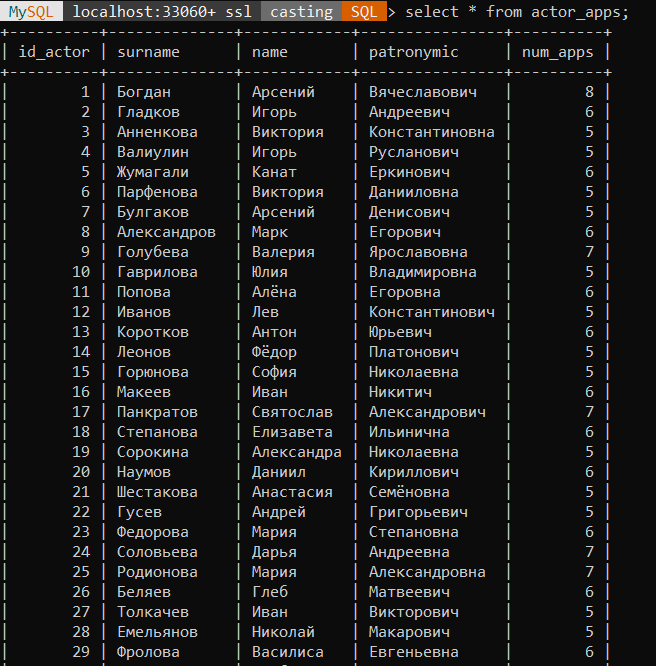
\includegraphics[width=0.9\linewidth]{pic5.png}
	\caption{Результат заполнения таблицы actor\_apps}
	\label{fig:pic5}
\end{figure}


После создания таблицы были созданы триггеры: 

\textbf{1. Триггер add\_app}
\begin{itemize}
	\item Событие: Добавление новой заявки.
	\item Действие: Обновление числа заявок в таблице actor\_apps.
	\item Принцип работы: при добавлении новой заявки в таблицу application срабатывает триггер, обновляющий количество заявок для соответствующего актера в таблице actor\_apps.
\end{itemize}


Код триггера представлен в \hyperref[lst:l6]{листинге 6}.

\begin{lstlisting}[caption={Код триггера add\_app}, label=lst:l6]
CREATE TRIGGER add_app
AFTER INSERT ON application
FOR EACH ROW
BEGIN
	UPDATE actor_apps
	SET num_apps = num_apps + 1
	WHERE id_actor = NEW.id_actor;
END;
\end{lstlisting}


Для демонстрации работы данного триггера добавим новую заявку актеру с id\_actor = 1 следующим образом:

\begin{lstlisting}
INSERT INTO application(filmography, photos, id_actor, id_role, 
			 id_casting_director, id_director) 
VALUES ("Начало, Оппенгеймер", "E:/Documents/Photos/actor/1", 1, 1, 1, 1); 
\end{lstlisting}


Результат работы триггера представлен на \hyperref[fig:pic6]{рисунке 6.}

\begin{figure}[H]
	\centering
	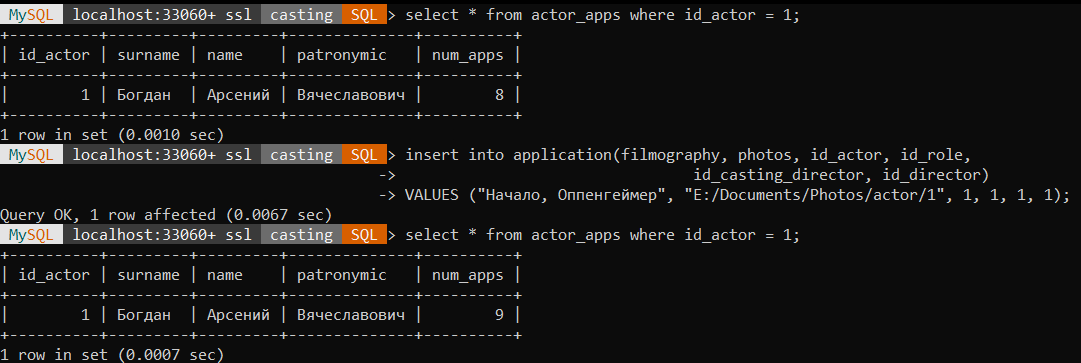
\includegraphics[width=1.0\linewidth]{pic6.png}
	\caption{Результат работы триггера add\_app}
	\label{fig:pic6}
\end{figure}





\textbf{2. Триггер delete\_app}
\begin{itemize}
	\item Событие: Удаление заявки.
	\item Действие: Обновление числа заявок в таблице actor\_apps.
	\item Принцип работы: при удалении заявки в таблице application срабатывает триггер, обновляющий количество заявок для соответствующего актера в таблице actor\_apps.
\end{itemize}

Код триггера представлен в \hyperref[lst:l7]{листинге 7}.
\newpage

\begin{lstlisting}[caption={Код триггера add\_app}, label=lst:l7]
CREATE TRIGGER delete_app
AFTER DELETE ON application
FOR EACH ROW
BEGIN
	UPDATE actor_apps
	SET num_apps = num_apps - 1
	WHERE id_actor = OLD.id_actor;
END;
\end{lstlisting}


Для демонстрации работы данного триггера удалим заявку актеру с id\_actor = 1. Для этого сначала нужно удалить все записи в других таблицах, которые ссылаются на первичный ключ таблицы application.

\begin{lstlisting}
DELETE FROM doubles_audition WHERE id_application = 1; 
DELETE FROM audition WHERE id_application = 1; 
DELETE FROM first_stage WHERE id_application = 1;
DELETE FROM application WHERE id_application = 1; 
\end{lstlisting}


Результат работы триггера представлен на \hyperref[fig:pic7]{рисунке 7.}

\begin{figure}[H]
	\centering
	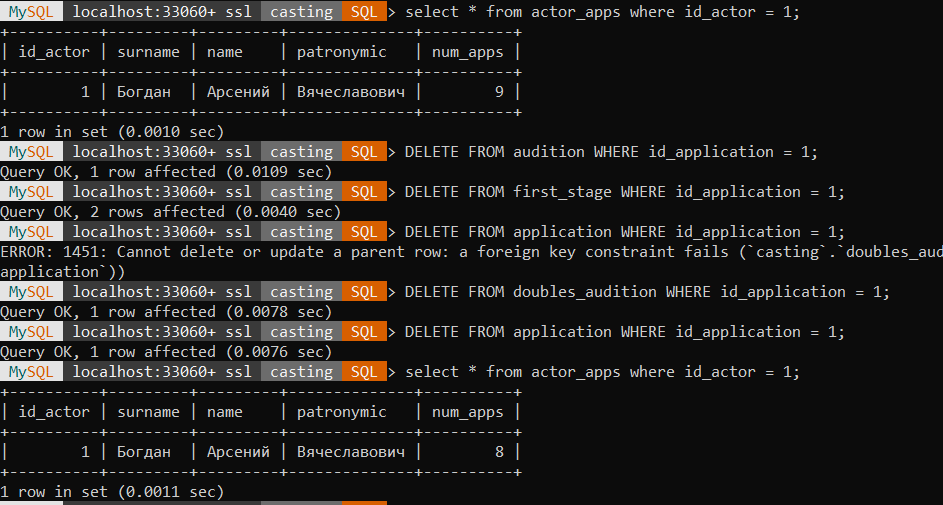
\includegraphics[width=1.0\linewidth]{pic7.png}
	\caption{Результат работы триггера delete\_app}
	\label{fig:pic7}
\end{figure}





\textbf{3. Триггер add\_actor}
\begin{itemize}
	\item Событие: Добавление нового актера в таблицу actor.
	\item Действие: Добавление данных нового актера в таблицу actor\_apps.
	\item Принцип работы: при добавлении нового актера в таблицу actor срабатывает триггер, добавляющий данные нового актера в таблицу actor\_apps.
\end{itemize}

Код триггера представлен в \hyperref[lst:l8]{листинге 8}.

\begin{lstlisting}[caption={Код триггера add\_actor}, label=lst:l8]
CREATE TRIGGER add_actor
AFTER INSERT ON actor
FOR EACH ROW
BEGIN
	INSERT INTO actor_apps (id_actor, surname, name, patronymic, num_apps)
	VALUES (NEW.id_actor, NEW.surname, NEW.name, NEW.patronymic, 0);
END;
\end{lstlisting}


Для демонстрации работы данного триггера добавим нового актера в таблицу actor.

\begin{lstlisting}
INSERT INTO actor(surname, name, patronymic, date_of_birth) 
VALUES ('Соловьев', 'Михаил', 'Владимирович', '2000-02-13'); 
\end{lstlisting}


Результат работы триггера представлен на \hyperref[fig:pic8]{рисунке 8.}

\begin{figure}[H]
	\centering
	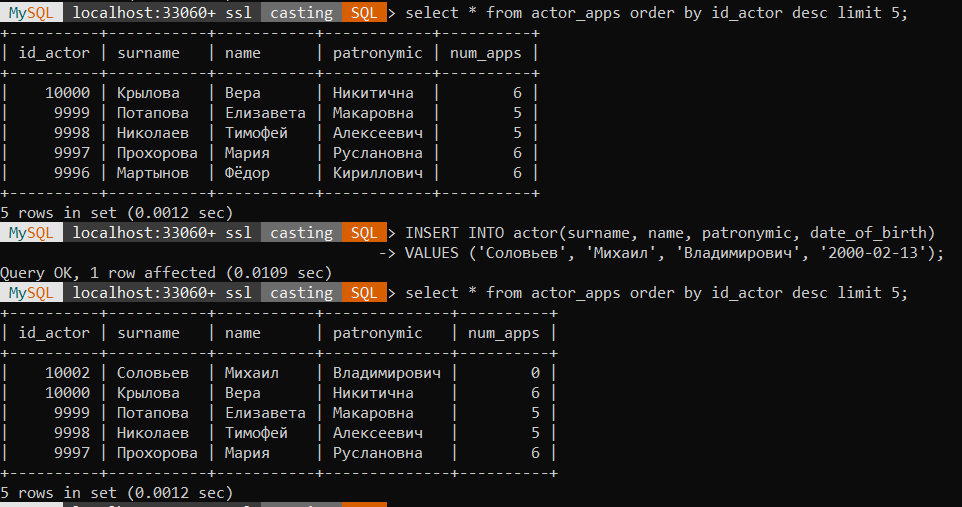
\includegraphics[width=0.9\linewidth]{pic8.png}
	\caption{Результат работы триггера add\_actor}
	\label{fig:pic8}
\end{figure}


\textbf{4. Триггер delete\_actor}
\begin{itemize}
	\item Событие: Удаление актера из таблицы actor.
	\item Действие: Удаление данных актера из таблицы actor\_apps.
	\item Принцип работы: при удалении актера из таблицы actor срабатывает триггер, удаляющий данные актера из таблицы actor\_apps.
\end{itemize}

Код триггера представлен в \hyperref[lst:l9]{листинге 9}.

\begin{lstlisting}[caption={Код триггера delete\_actor}, label=lst:l9]
CREATE TRIGGER delete_actor
AFTER DELETE ON actor
FOR EACH ROW
BEGIN
	DELETE FROM actor_apps
	WHERE id_actor = OLD.id_actor;
END;
\end{lstlisting}


Для демонстрации работы данного триггера удалим актера из таблицы actor.

\begin{lstlisting}
DELETE FROM actor WHERE id_actor = 10002;
\end{lstlisting}


Результат работы триггера представлен на \hyperref[fig:pic9]{рисунке 9.}

\begin{figure}[H]
	\centering
	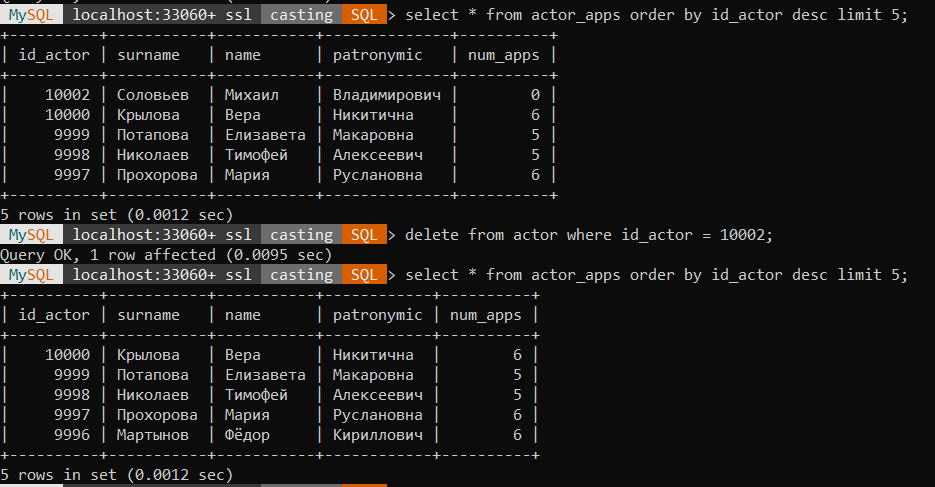
\includegraphics[width=0.9\linewidth]{pic9.png}
	\caption{Результат работы триггера delete\_actor}
	\label{fig:pic9}
\end{figure}




\textbf{5. Триггер update\_actor}
\begin{itemize}
	\item Событие: Обновление данных актера в таблице actor.
	\item Действие: Обновление данных актера в таблице actor\_apps.
	\item Принцип работы: при изменении данных актера в таблице actor срабатывает триггер, обновляющий данные актера в таблице actor\_apps.
\end{itemize}

Код триггера представлен в \hyperref[lst:l10]{листинге 10}.
\newpage
\begin{lstlisting}[caption={Код триггера update\_actor}, label=lst:l10]
CREATE TRIGGER update_actor
AFTER UPDATE ON actor
FOR EACH ROW
BEGIN
	UPDATE actor_apps
	SET surname = NEW.surname,
		name = NEW.name,
		patronymic = NEW.patronymic
	WHERE id_actor = NEW.id_actor;
END;	
\end{lstlisting}


Для демонстрации работы данного триггера изменим данные актера в таблице actor.

\begin{lstlisting}
UPDATE actor
SET 
	surname = 'Богдан',
	name = 'Арсений',
	patronymic = 'Вячеславович'
WHERE id_actor = 1;	
\end{lstlisting}

Результат работы триггера представлен на \hyperref[fig:pic10]{рисунке 10.}

\begin{figure}[H]
	\centering
	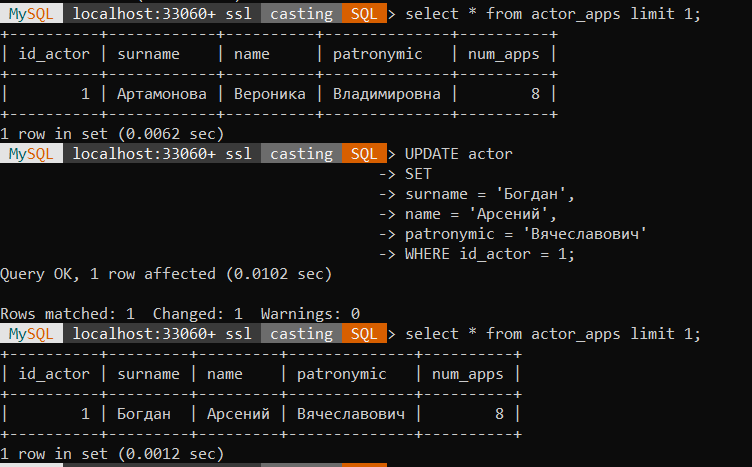
\includegraphics[width=0.9\linewidth]{pic10.png}
	\caption{Результат работы триггера update\_actor}
	\label{fig:pic10}
\end{figure}


\subsection{Разграничение прав доступа}

\textbf{Задача:} Создать двух пользователей. Первый должен уметь читать созданное ранее представление, а второй -- редактировать таблицы, участвующие в нем.

\par В результате реализации задачи было создано два пользователя - \textbf{reader} и \textbf{editor}. Первому пользователю предоставляются права только на чтение, второму -- на просмотр представления и редактирование таблиц представления director, film, role, application, actor.

Код создания пользователей и предоставление им прав представлен в \hyperref[lst:l11]{листинге 11}.

\begin{lstlisting}[caption={Код создания пользователей и назначения им прав}, label=lst:l11]
CREATE USER IF NOT EXISTS 'reader'@'localhost' IDENTIFIED BY '1111';
CREATE USER IF NOT EXISTS 'editor'@'localhost' IDENTIFIED BY '0000';

GRANT SELECT ON casting.director_view TO 'reader'@'localhost';

GRANT SELECT ON casting.director_view TO 'editor'@'localhost';

GRANT SELECT, INSERT, DELETE, UPDATE ON casting.film TO 'editor'@'localhost';
GRANT SELECT, INSERT, DELETE, UPDATE ON casting.role TO 'editor'@'localhost';
GRANT SELECT, INSERT, DELETE, UPDATE ON casting.application TO 'editor'@'localhost';
GRANT SELECT, INSERT, DELETE, UPDATE ON casting.actor TO 'editor'@'localhost';
\end{lstlisting}

Чтобы переключиться на другого пользователя используем команду в консоли:
\begin{lstlisting}
mysql -u editor -p -h localhost
\end{lstlisting}

В  \hyperref[tab:tb1]{таблице 1} представлено сравнение реакций на различные действия пользователей reader и editor.

\newpage
\begin{table}[H]
\caption{Сравнение реакций на различные действия}
\label{tab:tb1}

\begin{tabularx}{\textwidth}{|c|X|X|}
	\cline{1-3}
	\textbf{№} & \textbf{editor} & \textbf{reader} \\
	\cline{1-3}
	
	\multirow{3}{*}{1} & \multicolumn{2}{c|}{\textbf{Просмотр таблицы director\_view}}\\
	& \multicolumn{2}{c|}{SELECT * from director\_view;}\\
	\cline{2-3}
	& 
	\vspace{-6pt}
	\hspace{-8.5pt}
	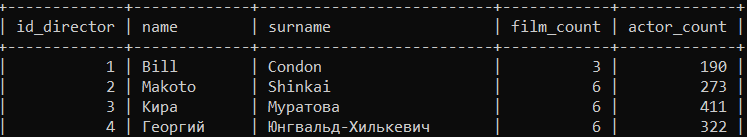
\includegraphics[width=1\linewidth]{n1.png}
	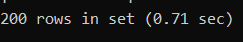
\includegraphics[width=1\linewidth]{e1.png}
	& 
	\vspace{-6pt}
	\hspace{-8.5pt}
	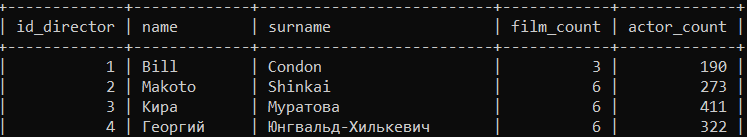
\includegraphics[width=1\linewidth]{n1.png}
	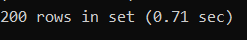
\includegraphics[width=1\linewidth]{r1.png}
	\\
	\cline{1-3}
	
	
	\multirow{3}{*}{2} & \multicolumn{2}{c|}{\textbf{Добавление в таблицу director}}\\
	& \multicolumn{2}{c|}{\parbox{0.85\linewidth}{INSERT INTO director(name, surname, date\_of\_birth) VALUES ('Кристофер', 'Нолан', 1970-07-30);}} \\
	\cline{2-3}
	& 
	\vspace{-6pt}
	\hspace{-8.5pt}
	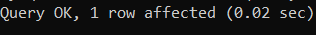
\includegraphics[width=1\linewidth]{e2.png}
	& 
	\vspace{-6pt}
	\hspace{-8.5pt}
	ERROR 1142 (42000): INSERT command denied to user 'reader'@'localhost' for table 'director'
	\\
	\cline{1-3}
	
	\multirow{3}{*}{3} & \multicolumn{2}{c|}{\textbf{Результат добавления в таблицу director}}\\
	& \multicolumn{2}{c|}{SELECT * FROM director ORDER BY id\_director DESC LIMIT 1;} \\
	\cline{2-3}
	& 
	\vspace{-6pt}
	\hspace{-8.5pt}
	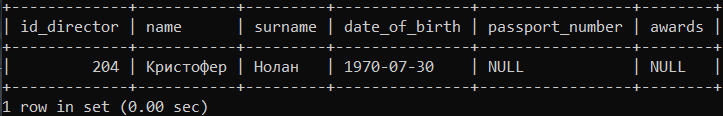
\includegraphics[width=1\linewidth]{n2.png}
	& 
	\vspace{-6pt}
	\hspace{-8.5pt}
	ERROR 1142 (42000): SELECT command denied to user 'reader'@'localhost' for table 'director'
	\\
	\cline{1-3}
	
	
	\multirow{3}{*}{4} & \multicolumn{2}{c|}{\textbf{Удаление из таблицы director}}\\
	& \multicolumn{2}{c|}{DELETE FROM director WHERE id\_director = 204;} \\
	\cline{2-3}
	& 
	\vspace{-6pt}
	\hspace{-8.5pt}
	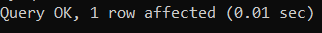
\includegraphics[width=1\linewidth]{e3.png}
	& 
	\vspace{-6pt}
	\hspace{-8.5pt}
	ERROR 1142 (42000): DELETE command denied to user 'reader'@'localhost' for table 'director'
	\\
	\cline{1-3}
	
	\multirow{3}{*}{5} & \multicolumn{2}{c|}{\textbf{Результат удаления из таблицы director}}\\
	& \multicolumn{2}{c|}{SELECT * FROM director WHERE id\_director = 204;} \\
	\cline{2-3}
	& 
	\vspace{-6pt}
	\hspace{-8.5pt}
	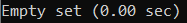
\includegraphics[width=1\linewidth]{n3.png}
	& 
	\vspace{-6pt}
	\hspace{-8.5pt}
	ERROR 1142 (42000): SELECT command denied to user 'reader'@'localhost' for table 'director'
	\\
	\cline{1-3}
	
	
	\multirow{3}{*}{6} & \multicolumn{2}{c|}{\textbf{Добавление записи в таблицу film}}\\
	& \multicolumn{2}{c|}{\parbox{0.85\linewidth}{INSERT INTO film(name, id\_director, id\_casting\_director) VALUES \\ ('Социальная сеть', 1, 1);}} \\
	\cline{2-3}
	& 
	\vspace{-6pt}
	\hspace{-8.5pt}
	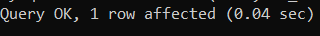
\includegraphics[width=1\linewidth]{e4.png}
	& 
	\vspace{-6pt}
	\hspace{-8.5pt}
	ERROR 1142 (42000): INSERT command denied to user 'reader'@'localhost' for table 'film'
	\\
	\cline{1-3}
	
	
	
\end{tabularx}
\end{table}




\newpage
\begin{table}[H]
	\label{tab:tb1}
	
	\begin{tabularx}{\textwidth}{|c|X|X|}
		\cline{1-3}
		\textbf{№} & \textbf{editor} & \textbf{reader} \\
		\cline{1-3}
		
		\multirow{3}{*}{7} & \multicolumn{2}{c|}{\textbf{Результат добавления записи в таблицу film}}\\
		& \multicolumn{2}{c|}{SELECT * FROM film ORDER BY id\_film DESC LIMIT 1;} \\
		\cline{2-3}
		& 
		\vspace{-6pt}
		\hspace{-8.5pt}
		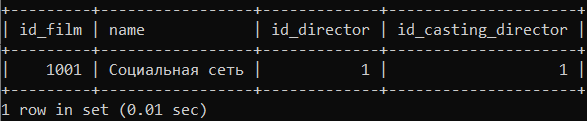
\includegraphics[width=1\linewidth]{n4.png}
		& 
		\vspace{-6pt}
		\hspace{-8.5pt}
		ERROR 1142 (42000): SELECT command denied to user 'reader'@'localhost' for table 'film'
		\\
		\cline{1-3}
		
		
		\multirow{3}{*}{8} & \multicolumn{2}{c|}{\textbf{Удаление записи из таблицы application}}\\
		& \multicolumn{2}{c|}{DELETE FROM application WHERE id\_application = 59995;} \\
		\cline{2-3}
		& 
		\vspace{-6pt}
		\hspace{-8.5pt}
		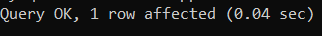
\includegraphics[width=1\linewidth]{e5.png}
		& 
		\vspace{-6pt}
		\hspace{-8.5pt}
		ERROR 1142 (42000): DELETE command denied to user 'reader'@'localhost' for table 'application'
		\\
		\cline{1-3}
		
		\multirow{3}{*}{9} & \multicolumn{2}{c|}{\textbf{Результат удаления записи из таблицы application}}\\
		& \multicolumn{2}{c|}{SELECT * FROM application WHERE id\_application = 59995;} \\
		\cline{2-3}
		& 
		\vspace{-6pt}
		\hspace{-8.5pt}
		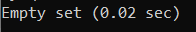
\includegraphics[width=1\linewidth]{n5.png}
		& 
		\vspace{-6pt}
		\hspace{-8.5pt}
		ERROR 1142 (42000): SELECT command denied to user 'reader'@'localhost' for table 'application'
		\\
		\cline{1-3}
		
		
		\multirow{3}{*}{10} & \multicolumn{2}{c|}{\textbf{Удаление таблицы actor}}\\
		& \multicolumn{2}{c|}{DROP table actor;} \\
		\cline{2-3}
		& 
		\vspace{-6pt}
		\hspace{-8.5pt}
		ERROR 1142 (42000): DROP command denied to user 'editor'@'localhost' for table 'actor'
		& 
		\vspace{-6pt}
		\hspace{-8.5pt}
		ERROR 1142 (42000): DROP command denied to user 'reader'@'localhost' for table 'actor'
		\\
		\cline{1-3}
		
		
		\multirow{3}{*}{11} & \multicolumn{2}{c|}{\textbf{Добавление записи в таблицу genres}}\\
		& \multicolumn{2}{c|}{INSERT INTO genres(name) VALUES ('Артхаус');} \\
		\cline{2-3}
		& 
		\vspace{-6pt}
		\hspace{-8.5pt}
		ERROR 1142 (42000): INSERT command denied to user 'editor'@'localhost' for table 'genres'
		& 
		\vspace{-6pt}
		\hspace{-8.5pt}
		ERROR 1142 (42000): INSERT command denied to user 'reader'@'localhost' for table 'genres'
		\\
		\cline{1-3}
	
				
		\multirow{3}{*}{12} & \multicolumn{2}{c|}{\textbf{Изменение таблицы role}}\\
		& \multicolumn{2}{c|}{UPDATE role SET name = 'Шерлок Холмс' WHERE id\_role = 1;}\\
		\cline{2-3}
		& 
		\vspace{-6pt}
		\hspace{-8.5pt}
		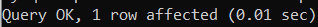
\includegraphics[width=1\linewidth]{e6.png}
		& 
		\vspace{-6pt}
		\hspace{-8.5pt}
		ERROR 1142 (42000): UPDATE command denied to user 'reader'@'localhost' for table 'role'
		\\
		\cline{1-3}
		
		\multirow{3}{*}{13} & \multicolumn{2}{c|}{\textbf{Результат изменения записи в таблице role}}\\
		& \multicolumn{2}{c|}{SELECT * FROM role WHERE id\_role = 1;}\\
		\cline{2-3}
		& 
		\vspace{-6pt}
		\hspace{-8.5pt}
		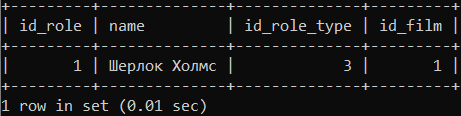
\includegraphics[width=1\linewidth]{n6.png}
		& 
		\vspace{-6pt}
		\hspace{-8.5pt}
		ERROR 1142 (42000): SELECT command denied to user 'reader'@'localhost' for table 'role'
		\\
		\cline{1-3}
		
		
	\end{tabularx}
\end{table}


\newpage
\subsection{Функции и процедуры}

\subsubsection{Функция}

\textbf{Задача:} Реализовать функцию, принимающую в качестве аргументов фамилию, имя и отчество и возвращающую строку формата "Фамилия.И.О."

Код создания функции представлен в \hyperref[lst:l12]{листинге 12}.

\begin{lstlisting}[caption={Код создания функции GetFullName}, label=lst:l12]
DELIMITER //
CREATE FUNCTION GetFullName (
	surname VARCHAR(30), 
	name VARCHAR(20),
	patronymic VARCHAR(20)
) RETURNS VARCHAR(35)
DETERMINISTIC
BEGIN 
	RETURN CONCAT(
	LEFT(name, 1), '.', 
	IF(patronymic IS NOT NULL, CONCAT(LEFT(patronymic, 1), '.'), ''),
	surname
);
END //

DELIMITER ;

\end{lstlisting}

Пример использования функции: 

\begin{lstlisting}
SELECT surname, name, patronymic, 
	GetFullName(surname, name, patronymic) as full_name
FROM actor 
LIMIT 5;
\end{lstlisting}

Результат выполнения запроса с использованием фукнции представлен на \hyperref[fig:pic11]{рисунке 11.}

\begin{figure}[H]
	\centering
	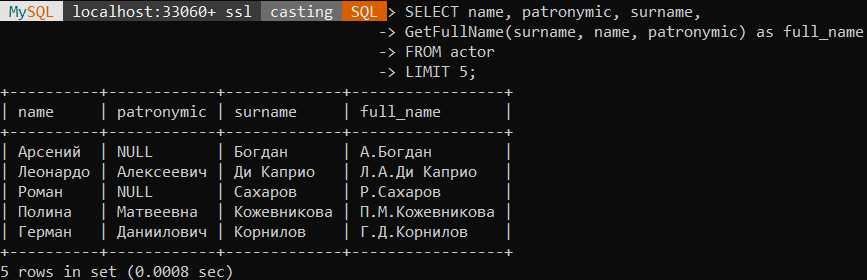
\includegraphics[width=1.0\linewidth]{pic11.png}
	\caption{Результат выполнения запроса с функцией}
	\label{fig:pic11}
\end{figure}

Если же вызвать функцию и передать попробовать ей атрибуты, которых нет в таблице, то получим ошибку. Пример такого ошибочного использования представлен ниже, а результат его выполнения на \hyperref[fig:pic12]{рисунке 12.}
\begin{lstlisting}
	SELECT GetFullName(surname, name, patronymic) as full_name
	FROM application 
	LIMIT 5;
\end{lstlisting}

\begin{figure}[H]
	\centering
	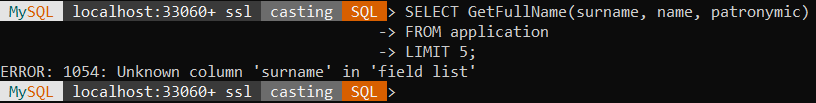
\includegraphics[width=1.0\linewidth]{pic12.png}
	\caption{Результат выполнения запроса}
	\label{fig:pic12}
\end{figure}

\subsubsection{Процедура}

\textbf{Задача:} Реализовать процедуру, добавляющую новую запись в таблицу application и принимающую в качестве аргументов фамилию, имя, отчество, дату рождения, номер паспорта, образование и опыт работы актера, а также имя, фамилия, дату рождения, номер паспорта и награды режиссера, id кастинг-директора и id роли. При вызове процедуры проверять, существует ли запись в таблице actor с такими же фамилией, именем и отчеством, и, если она существует, при необходимости обновить значения полей записи.  

Код создания функции представлен в \hyperref[lst:l13]{листинге 13}.

\begin{lstlisting}[caption={Код создания процедуры new\_application}, label=lst:l13, language=sql]
DELIMITER // 

CREATE PROCEDURE new_application(
	IN ac_surname varchar(30),
	IN ac_name varchar(20), 
	IN ac_patronymic varchar(20),    
	IN ac_date_of_birth date, 
	IN ac_passport_number varchar(15),
	IN ac_education varchar(100),
	IN ac_work_experience varchar(100),
	IN d_surname varchar(30),
	IN d_name varchar(20), 
	IN d_date_of_birth date, 
	IN d_passport_number varchar(15),
	IN d_awards varchar(100),
	IN id_cas_dir int unsigned,
	IN id_input_role int unsigned
)
BEGIN
	DECLARE act_id INT DEFAULT NULL;
	DECLARE dir_id INT DEFAULT NULL;
	
	SELECT id_actor INTO act_id
		FROM actor
		WHERE surname = ac_surname COLLATE utf8mb4_unicode_ci
		AND name = ac_name COLLATE utf8mb4_unicode_ci
		AND patronymic = ac_patronymic COLLATE utf8mb4_unicode_ci
		AND date_of_birth = ac_date_of_birth;
	
	IF act_id IS NULL THEN
		INSERT INTO actor(surname, name, patronymic, date_of_birth, 
						passport_number, education, work_experience)
		VALUES(ac_surname, ac_name, ac_patronymic, ac_date_of_birth,
				ac_passport_number, ac_education, ac_work_experience);
		SET act_id = LAST_INSERT_ID();
	
	ELSEIF EXISTS (SELECT 1 FROM actor WHERE id_actor = act_id
		AND (passport_number <> ac_passport_number
		OR education <> ac_education
		OR work_experience <> ac_work_experience)
	) THEN
		UPDATE actor
		SET passport_number = ac_passport_number, education = ac_education, 
		work_experience = ac_work_experience WHERE id_actor = act_id;
	END IF;
	
	SELECT id_director INTO dir_id
		FROM director
		WHERE surname = d_surname COLLATE utf8mb4_unicode_ci
		AND name = d_name COLLATE utf8mb4_unicode_ci
		AND date_of_birth = d_date_of_birth;
	
	IF dir_id IS NULL THEN
		INSERT INTO director(surname, name, date_of_birth, passport_number, awards)
		VALUES(d_surname, d_name, d_date_of_birth, d_passport_number, d_awards);
		SET dir_id = LAST_INSERT_ID();
	ELSEIF EXISTS (SELECT 1 FROM director WHERE id_director = dir_id
		AND (passport_number <> d_passport_number
		OR awards <> d_awards)
	) THEN
		UPDATE director
		SET passport_number = d_passport_number, awards = d_awards 
		WHERE id_director = dir_id;
	END IF;
	
	-- Вставка в таблицу application
	INSERT INTO application(filmography, photos, id_actor, id_role, id_casting_director, id_director)
	VALUES(NULL, NULL, act_id, id_input_role, id_cas_dir, dir_id);

END //

DELIMITER ;
\end{lstlisting}

Продемонстрируем результаты работы процедуры для следующих случаев:
\begin{enumerate}
	\item Актер и режиссер уже существуют в таблицах actor и director, но некоторые их данные \textbf{НЕ совпадают} с входными значениями аргументов процедуры;
	\item Актер и режиссер уже существуют в таблицах actor и director, и все данные \\ \textbf{совпадают} с входными значениями аргументов вызываемой процедуры;
	\item Актера и режиссера \textbf{не существует} в таблицах actor и director до вызова процедуры.
\end{enumerate}

\paragraph{Первый пример}

Для демонстрации \textbf{первого} примера, сначала посмотрим, какие заявки имеются у актера с id\_actor = 2. Для этого выполним следующий запрос: 

\begin{lstlisting}
SELECT a.id_actor, a.surname, a.name, app.id_application, 
	r.id_role, dir.id_director
FROM actor a
LEFT JOIN application app on a.id_actor = app.id_actor
JOIN director dir on app.id_director = dir.id_director
JOIN role r on app.id_role = r.id_role
WHERE a.id_actor = 2;
\end{lstlisting}

Также выполним запросы для просмотра всей информации об актере и режиссере:
\begin{lstlisting}
SELECT * from actor where id_actor = 2;

SELECT * from director where id_director = 54;
\end{lstlisting}

Результаты выполнения запросов представлены на \hyperref[fig:pic13]{рисунках 13-15.}
\newpage
\begin{figure}[H]
	\centering
	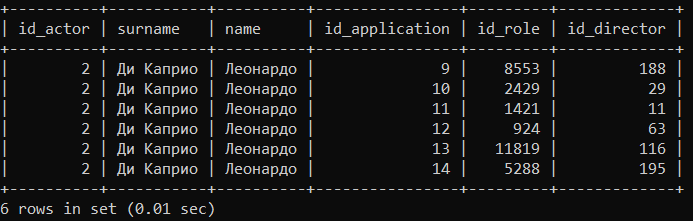
\includegraphics[width=0.9\linewidth]{pic13.png}
	\caption{Данные о заявках актера}
	\label{fig:pic13}
\end{figure}

\begin{figure}[H]
	\centering
	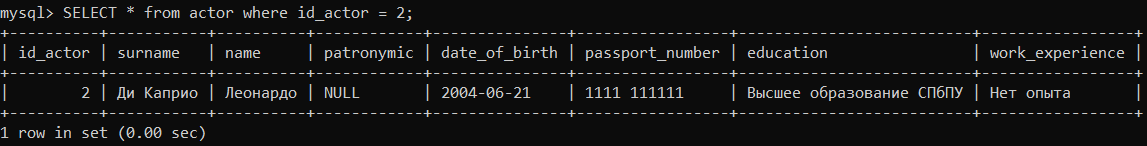
\includegraphics[width=1.0\linewidth]{pic15.png}
	\caption{Данные актера}
	\label{fig:pic14}
\end{figure}

\begin{figure}[H]
	\centering
	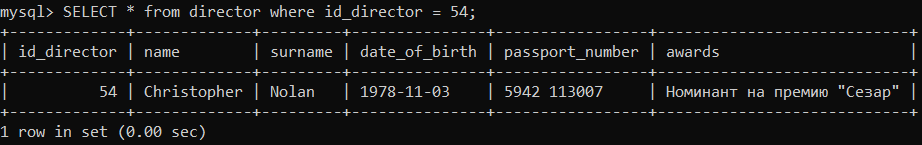
\includegraphics[width=1.0\linewidth]{pic14.png}
	\caption{Данные режиссера}
	\label{fig:pic15}
\end{figure}


\textbf{Теперь вызовем процедуру:} 

\begin{lstlisting}
CALL new_application(
	'Ди Каприо', 'Леонардо', 'Алексеевич', '2004-06-21',        
	'1234567890', 'СПбПУ + Oxford',
	'Снялся в фильме Титаник',       
	'Nolan', 'Christopher', '1978-11-03', '0987654321',        
	'Оскар (лучший актер)',
	1, 1                   
);
\end{lstlisting}

Теперь посмотрим на результат, выполнив запросы, уже показанные выше. Результат представлен на  \hyperref[fig:pic14]{рисунках 16-18.}

\newpage

\begin{figure}[H]
	\centering
	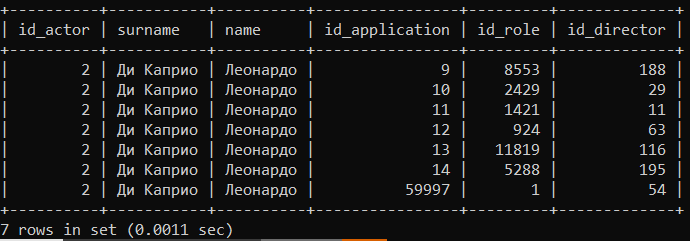
\includegraphics[width=1.0\linewidth]{pic16.png}
	\caption{Данные о заявках актера}
	\label{fig:pic16}
\end{figure}

\begin{figure}[H]
	\centering
	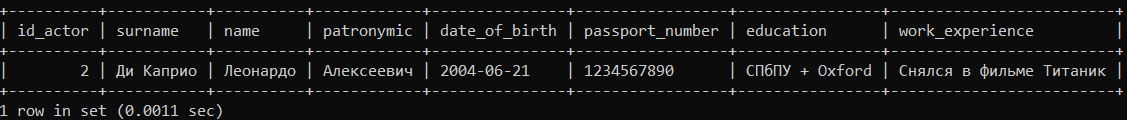
\includegraphics[width=1.0\linewidth]{pic17.png}
	\caption{Данные актера}
	\label{fig:pic17}
\end{figure}

\begin{figure}[H]
	\centering
	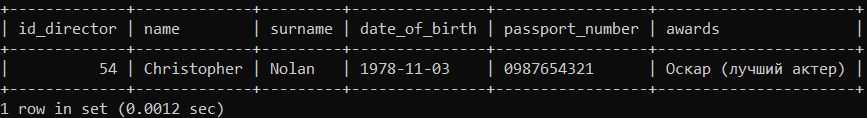
\includegraphics[width=1.0\linewidth]{pic18.png}
	\caption{Данные режиссера}
	\label{fig:pic18}
\end{figure}

\paragraph{Второй пример}

Для демонстрации \textbf{второго} случая изменим в вызове процедуры id\_role=2 и id\_casting\_director=2: 

\begin{lstlisting}
	CALL new_application(
	'Ди Каприо', 'Леонардо', 'Алексеевич', '2004-06-21', '1234567890',        
	'СПбПУ + Oxford',
	'Снялся в фильме Титаник',       
	'Nolan', 'Christopher',       
	'1978-11-03',  
	'0987654321',        
	'Оскар (лучший актер)',
	1, 1                   
	);
\end{lstlisting}

Результат выполнения процедуры представлен на \hyperref[fig:pic19]{рисунке 19.}

\begin{figure}[H]
	\centering
	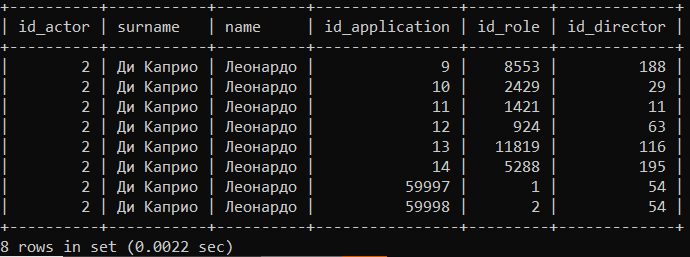
\includegraphics[width=1.0\linewidth]{pic19.png}
	\caption{Данные о заявках актера}
	\label{fig:pic19}
\end{figure}

\paragraph{Третий пример}

Для демонстрации \textbf{третьего} случая вызовем процедуру, указав новые данные актера и режиссера:

\begin{lstlisting}
CALL new_application(
	'Дауни-младший', 'Роберт', '', '1965-04-04', '1234567890',        
	'Cambridge University',
	'Снялся в Шерлок Холмсе',       
	'Квентин', 'Тарантино', '1978-11-03', '0987654321',        
    'Золотой глобус', 10, 10                   
);
\end{lstlisting}

Для демонстрации результатов выполнения процедуры просмотрим последнюю запись из таблиц actor и director, а также просмотрим дополнительную информацию о заявках нового актера.\hyperref[fig:pic20]{(рис. 20-22).}

\begin{figure}[H]
	\centering
	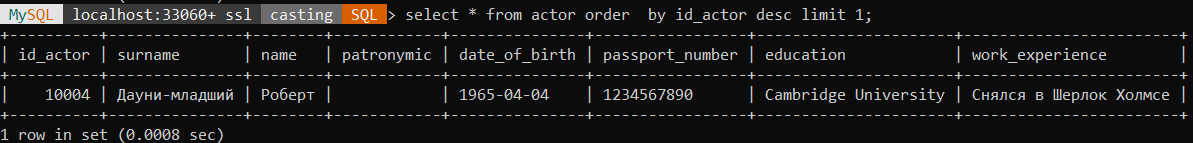
\includegraphics[width=1.0\linewidth]{pic20.png}
	\caption{Данные нового добавленного актера}
	\label{fig:pic20}
\end{figure}

\begin{figure}[H]
	\centering
	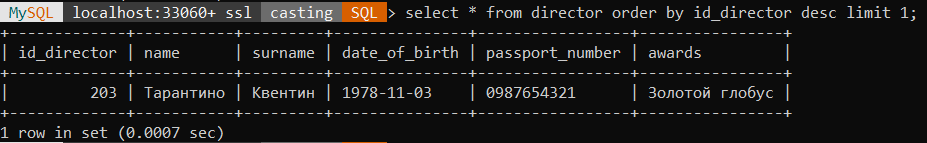
\includegraphics[width=1.0\linewidth]{pic21.png}
	\caption{Данные нового добавленного режиссера}
	\label{fig:pic22}
\end{figure}

\newpage
\begin{figure}[H]
	\centering
	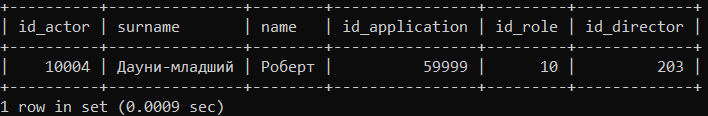
\includegraphics[width=1.0\linewidth]{pic22.png}
	\caption{Данные о заявках добавленного актера}
	\label{fig:pic21}
\end{figure}

\subsection{Транзакции}

\textbf{Задача:} Проверить уровень изоляции READ COMMITTED на наличие неповторяющихся и фантомных чтений.

\par READ COMMITTED — это уровень изоляции транзакций, при котором каждая транзакция видит только те изменения, которые уже были зафиксированы другими транзакциями. При таком уровне изоляции возможны две основные проблемы: неповторяющиеся и фантомные чтения. 

\textbf{Проверим возникновение фантомного чтения}
\par Результат проведения транзакций представлен в \hyperref[tab:tb2]{таблице 2.} 


\begin{table}[H]
	\caption{Проведение транзакций}
	\label{tab:tb2}
	
	\begin{tabularx}{\textwidth}{|c|X|X|}
		\cline{1-3}
		\textbf{№} & \textbf{Транзакция №1} & \textbf{Транзакция №2} \\
		\cline{1-3}
		
		\multirow{3}{*}{1} & \multicolumn{2}{c|}{Установка уровня изоляции на READ COMMITTED}\\
		\cline{2-3}
		& 
		\vspace{-6pt}
		\hspace{-5pt}
		{\parbox{0.85\linewidth}{SET SESSION TRANSACTION ISOLATION LEVEL READ COMMITTED;}}
		& 
		\vspace{-6pt}
		\hspace{-5pt}
		{\parbox{0.85\linewidth}{SET SESSION TRANSACTION ISOLATION LEVEL READ COMMITTED;}}
		\\
		\cline{1-3}
		
		
		
		
		\multirow{3}{*}{1} & \multicolumn{2}{c|}{Начало транзакций}\\
		\cline{2-3}
		& 
		\vspace{-6pt}
		\hspace{-5pt}
		\textbf{START TRANSACTION;}
		& 
		\vspace{-6pt}
		\hspace{-5pt}
		\textbf{START TRANSACTION;}
		\\
		\cline{1-3}
		
		\multirow{3}{*}{2} & \multicolumn{2}{c|}{Читаем значения из таблицы role\_type}\\
		\cline{2-3}
		& 
		\vspace{-6pt}
		\hspace{-8.5pt}
		\textbf{SELECT * FROM role\_type;}
		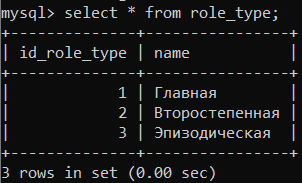
\includegraphics[width=1\linewidth]{pic23.png}
		& 
		\vspace{-6pt}
		\hspace{-8.5pt}
		\\
		\cline{1-3}
		
		
	\end{tabularx}
\end{table}		


\newpage
\begin{table}[H]
	\label{tab:tb2}
	
	\begin{tabularx}{\textwidth}{|c|X|X|}
		\cline{1-3}
		\textbf{№} & \textbf{Транзакция №1} & \textbf{Транзакция №2} \\
		\cline{1-3}
		
		\multirow{3}{*}{3} & \multicolumn{2}{c|}{Добавляем новую запись в таблицу role\_type и сохраняем результат}\\
		\cline{2-3}
		& 
		\vspace{-6pt}
		\hspace{-5pt}
		& 
		\vspace{-6pt}
		\hspace{-5pt}
		\textbf{INSERT INTO role\_type(name) VALUES('Камео');}
		\\
		\cline{1-3}
		
		\multirow{3}{*}{3} & \multicolumn{2}{c|}{Проверим добавление новой записи в таблицу role\_type}\\
		\cline{2-3}
		& 
		\vspace{-6pt}
		\hspace{-5pt}
		& 
		\vspace{-6pt}
		\hspace{-5pt}
		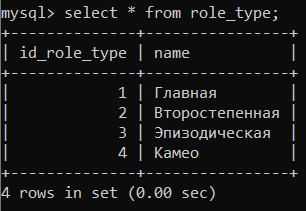
\includegraphics[width=1\linewidth]{pic24.png}
		\\
		\cline{1-3}
		
		\multirow{3}{*}{3} & \multicolumn{2}{c|}{Фиксируем внесенные изменения}\\
		\cline{2-3}
		& 
		\vspace{-6pt}
		\hspace{-5pt}
		& 
		\vspace{-6pt}
		\hspace{-5pt}
		\textbf{COMMIT;}
		\\
		\cline{1-3}
		
		
		\multirow{3}{*}{4} & \multicolumn{2}{c|}{Читаем значения из таблицы role\_type и получаем фантомное чтение}\\
		\cline{2-3}
		& 
		\vspace{-6pt}
		\hspace{-8.5pt}
		\textbf{SELECT * FROM role\_type;}
		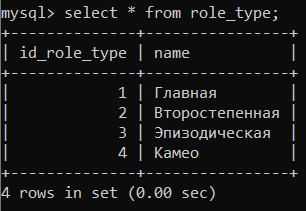
\includegraphics[width=1\linewidth]{pic24.png}
		& 
		\vspace{-6pt}
		\hspace{-8.5pt}
		\\
		\cline{1-3}
		
	\end{tabularx}
\end{table}		
		
\par Таблица иллюстрирует выполнение транзакций при уровне изоляции READ COMMITTED. Сначала устанавливается уровень изоляции, затем обе транзакции начинают выполнение. Транзакция №2 добавляет запись в таблицу role\_type, после чего фиксирует изменения. Транзакция №1, выполняя повторное чтение данных, обнаруживает \textbf{фантомное чтение}, когда новая запись становится видимой, добавленная другой транзакцией, хотя в момент первоначального чтения эти данные не существовали.	


\newpage
\section*{Заключение}
\addcontentsline{toc}{section}{Заключение}

В ходе курсовой работы были выполнены 5 лабораторных работ.
\begin{enumerate}
	\item Создано представление, в котором для каждого режиссера подсчитывается общее количество его фильмов и актеров, участвующих в его фильмах. Также было написано два запроса, добавляющие к представлению новую информацию: общее количество жанров и ролей в фильмах каждого режиссера и количество утвержденных заявок для фильмов каждого режиссера. Количество записей в представлении: 200. 
	
	\item Написаны 5 триггеров, поддерживающие целостность данных созданной таблицы, в которой для каждого актера подсчитывается число заявок. Количество записей в созданной таблице: 10002.
	
	\item Созданы два пользователя: reader и editor. Первый имеет доступ только на просмотр представления, а второй также может редактировать таблицы, из которых оно состоит.
	
	\item Написаны функция и процедура. Функция принимает в качестве аргументов фамилию, имя и отчество и возвращает строку формата "Фамилия И. О.". Процедура принимает в качестве аргументов фамилию, имя, отчество, дату рождения, номер паспорта, образование и опыт работы актера, а также имя, фамилия, дату рождения, номер паспорта и награды режиссера, id кастинг-директора и id роли. При вызове процедуры, если данные об актере и режиссере отсутствуют, должны создаваться соответствующие записи в таблицах actor и director. Если же данные об актере и режиссере есть, но с изменениями в некоторых полях, применяет новые изменения. После в таблице application создается новая запись с id соответствующих записей. 
	
	\item Проведена демонстрация возможности наличия фантомного чтения на уровне READ COMMITTED. Для этого были запущены две транзакции с разных пользователей, работающие одновременно с одной таблице role\_type.
	
\end{enumerate}

В процессе выполнения лабораторных работ было написано 32 запроса. Для наглядного иллюстрирования процесса работы и результатов каждого задания суммарно в отчёте представлено 22 рисунка, 13 листингов и 2 таблицы. Времени потрачено на выполнение всех заданий вместе с написанием отчета на языке разметки LaTeX: 30 часов. 




\newpage
\section*{Список литературы}
\addcontentsline{toc}{section}{Список литературы} % Добавляем раздел в содержание

\begin{enumerate}[label={[\arabic*]}]
\item Мана Такахаси, Сёко Адзума. Базы данных. - Москва: ДМК Пресс, 2015. - 240 с.

\item Силверман, Бен. MySQL. Библия пользователя. - М.: ДМК Пресс, 2019. - 928 с.

\item Бейли, Ларри Ульман. Изучаем MySQL. - 3-е издание. - СПб.: Питер, 2019. - 736 с.

\end{enumerate}



\end{document}